%%%%%%%%%%%%%%%%%%%%%%%%%%%%%%%%%%%%%%%%%
% Jacobs Landscape Poster
% LaTeX Template
% Version 1.1 (14/06/14)
%
% Created by:
% Computational Physics and Biophysics Group, Jacobs University
% https://teamwork.jacobs-university.de:8443/confluence/display/CoPandBiG/LaTeX+Poster
% 
% Further modified by:
% Nathaniel Johnston (nathaniel@njohnston.ca)
%
% This template has been downloaded from:
% http://www.LaTeXTemplates.com
%
% License:
% CC BY-NC-SA 3.0 (http://creativecommons.org/licenses/by-nc-sa/3.0/)
%
%%%%%%%%%%%%%%%%%%%%%%%%%%%%%%%%%%%%%%%%%

%----------------------------------------------------------------------------------------
%	PACKAGES AND OTHER DOCUMENT CONFIGURATIONS
%----------------------------------------------------------------------------------------

\documentclass[final]{beamer}

\usepackage[scale=1.24]{beamerposter} % Use the beamerposter package for laying out the poster

\usetheme{confposter} % Use the confposter theme supplied with this template

\setbeamercolor{block title}{fg=ngreen,bg=white} % Colors of the block titles
\setbeamercolor{block body}{fg=black,bg=white} % Colors of the body of blocks
\setbeamercolor{block alerted title}{fg=white,bg=dblue!70} % Colors of the highlighted block titles
\setbeamercolor{block alerted body}{fg=black,bg=dblue!10} % Colors of the body of highlighted blocks
% Many more colors are available for use in beamerthemeconfposter.sty

%-----------------------------------------------------------
% Define the column widths and overall poster size
% To set effective sepwid, onecolwid and twocolwid values, first choose how many columns you want and how much separation you want between columns
% In this template, the separation width chosen is 0.024 of the paper width and a 4-column layout
% onecolwid should therefore be (1-(# of columns+1)*sepwid)/# of columns e.g. (1-(4+1)*0.024)/4 = 0.22
% Set twocolwid to be (2*onecolwid)+sepwid = 0.464
% Set threecolwid to be (3*onecolwid)+2*sepwid = 0.708

\newlength{\sepwid}
\newlength{\onecolwid}
\newlength{\twocolwid}
\newlength{\threecolwid}
% \setlength{\paperwidth}{36in} % A0 width: 46.8in
% \setlength{\paperheight}{48in} % A0 height: 33.1in
% \setlength{\sepwid}{0.024\paperwidth} % Separation width (white space) between columns
% \setlength{\onecolwid}{0.22\paperwidth} % Width of one column
% \setlength{\twocolwid}{0.464\paperwidth} % Width of two columns
% \setlength{\threecolwid}{0.708\paperwidth} % Width of three columns
% \setlength{\topmargin}{-0.5in} % Reduce the top margin size
\setlength{\paperwidth}{46.8in} % A0 width: 46.8in
\setlength{\paperheight}{33.1in} % A0 height: 33.1in
\setlength{\sepwid}{0.025\paperwidth}
\setlength{\onecolwid}{0.3\paperwidth}
\setlength{\twocolwid}{0.625\paperwidth}
\setlength{\topmargin}{-1in}
%-----------------------------------------------------------

\usepackage{graphicx}  % Required for including images
\usepackage{booktabs} % Top and bottom rules for tables

%----------------------------------------------------------------------------------------
%	TITLE SECTION 
%----------------------------------------------------------------------------------------

\title{\LARGE{CyberWallE at SemEval-2020 Task 11: An Analysis of}\\
\Huge{Feature Engineering} \huge{for} \Huge{Ensemble Models} \huge{for} \Huge{Propaganda Detection}}

\author{Verena Blaschke, Maxim Korniyenko and Sam Tureski}

\institute{Eberhard Karls Universität Tübingen\\
\href{https://github.com/cicl-iscl/CyberWallE-propaganda-detection}{\color{jblue} https://github.com/cicl-iscl/CyberWallE-propaganda-detection}
\qquad {first.last@student.uni-tuebingen.de}}

%----------------------------------------------------------------------------------------

%%%%%%%%% CUSTOM CHANGES

\newlength{\doublecoltopmargin}
\newlength{\singlecoltopmargin}
\setlength{\doublecoltopmargin}{-1.2in}
\setlength{\singlecoltopmargin}{-0.5in}


\setbeamertemplate{headline}{
 \leavevmode
  \begin{columns}
   \begin{column}{\linewidth}
    \vskip1cm
    \centering
    \usebeamercolor{title in headline}{\color{jblue}\Huge{\textbf{\inserttitle}}\\[0.5ex]}
    \usebeamercolor{author in headline}{\color{fg}\Large{\insertauthor}\\[1ex]}
    \usebeamercolor{institute in headline}{\color{fg}\large{\insertinstitute}\\[1ex]}
    \vskip1cm
   \end{column}
   \vspace{1cm}
  \end{columns}
  % reduce vspace
%  \vspace{0.2in}
 % change rule width match A0 format
 \hspace{0.7in}
 \begin{beamercolorbox}[wd=45.4in,colsep=0.15cm]{cboxb}\end{beamercolorbox}
 \vspace{0.1in}
}

\setlength\labelsep   {\dimexpr\labelsep + 1em\relax}

\setbeamerfont{block body}{series=\sffamily, size=\large}
\setbeamerfont{normal text}{series=\sffamily, size=\large}
\setbeamerfont{item}{series=\sffamily, size=\large}
\setbeamerfont{theorem title}{series=\sffamily, size=\large}

\setbeamercolor{bibliography entry title}{fg=black}
\setbeamercolor{bibliography entry location}{fg=black} 
\setbeamercolor{bibliography entry note}{fg=black}  
\setbeamertemplate{bibliography entry article}{}
\setbeamertemplate{bibliography entry title}{}
\setbeamertemplate{bibliography entry location}{}
\setbeamertemplate{bibliography entry note}{}

\definecolor{paleblue}{RGB}{240, 248, 255}
% \definecolor{turquoise}{RGB}{74, 186, 186}
\definecolor{turquoise}{RGB}{67, 171, 171}
\definecolor{paleyellow}{RGB}{252, 240, 146}
\definecolor{darkorange}{RGB}{250, 127, 77}
\definecolor{paleorange}{RGB}{240, 187, 165}

\setbeamercolor{item}{fg=turquoise}
\setbeamercolor{item projected}{fg=white,bg=turquoise}
\setbeamercolor{block title}{fg=turquoise,bg=white}

\setbeamercolor{block body example}{bg=gray!10}
\setbeamercolor{block title example}{bg=gray!20}

\setbeamertemplate{block alerted begin}
{
  \par\vskip\medskipamount
  \begin{beamercolorbox}[colsep*=0ex,dp={2ex},center]{block title}
    \vskip-0.75em
    \large\insertblocktitle
    \begin{flushleft}
    \vskip-1.5em
    \end{flushleft}
  \end{beamercolorbox}
  {\parskip0pt\par}
%   \ifbeamercolorempty[bg]{block title}
%   {}
%   {\ifbeamercolorempty[bg]{block body}{}{\nointerlineskip\vskip-0.5pt}}
  \usebeamerfont{block body}
  \vskip-0.5cm
  \begin{beamercolorbox}[colsep*=0ex,vmode]{block body}
  \justifying
}
\setbeamertemplate{block alerted end}
{
  \end{beamercolorbox}
  \vskip\smallskipamount
}

% https://tex.stackexchange.com/a/103256
\setbeamertemplate{itemize/enumerate body begin}{\setlength{\leftmargini}{0pt}}
\makeatletter
\addtobeamertemplate{block begin}{
\def\@listi{\leftmargin1.5em
  \topsep 3\p@ \@plus2\p@ \@minus2.5\p@
  \parsep 0\p@
  \itemsep3\p@ \@plus2\p@ \@minus3\p@}
}
\makeatother

% https://tex.stackexchange.com/questions/41683/why-is-it-that-coloring-in-soul-in-beamer-is-not-visible/41693#41693
\usepackage{soul}
\makeatletter
\let\HL\hl
\renewcommand\hl{%
  \let\set@color\beamerorig@set@color
  \let\reset@color\beamerorig@reset@color
  \HL}
\makeatother

% https://tex.stackexchange.com/questions/128064/how-to-overbrace-underbrace-in-text-mode-using-tikz
\newcommand{\undertext}[2] {$\underbrace{\textsf{#1}}_{\textsf{#2}}$}
\newcommand{\overtext}[2] {$\overbrace{\textsf{#1}}^{\textsf{#2}}$}
%----------------------------------------------------------------------------------------

\begin{document}
\addtobeamertemplate{block end}{}{\vspace*{2ex}} % White space under blocks
\addtobeamertemplate{block alerted end}{}{\vspace*{2ex}} % White space under highlighted (alert) blocks
\setlength{\belowcaptionskip}{2ex} % White space under figures
\setlength\belowdisplayshortskip{2ex} % White space under equations

\begin{frame}[t] % The whole poster is enclosed in one beamer frame
\begin{columns}[t] % The whole poster consists of three major columns - the [t] option aligns each column's content to the top
\begin{column}{\sepwid}\end{column} % Empty spacer column
\begin{column}{\twocolwid} % Begin a column which is two columns wide 
\begin{columns}[t,totalwidth=\twocolwid] % Split up the two columns wide column 
\begin{column}{\onecolwid}\vspace{\doublecoltopmargin} % The first column 

\begin{block}{Introduction}
Shared task \cite{DaSanMartinoSemeval20task11} to automatically
\begin{itemize}
    \item find propagandistic snippets in news articles
    \item determine which of 14 propaganda techniques is used in each such fragment
\end{itemize}
% 14 techniques total, the 3 largest: loaded language, name calling or labelling, repetition
\end{block}

%------------------------------------------------
\begin{block}{Finding propagandistic spans}
\begin{columns}[t,totalwidth=\onecolwid]
\begin{column}{0.145\paperwidth}
\vspace{-2.2em}
\begin{figure}
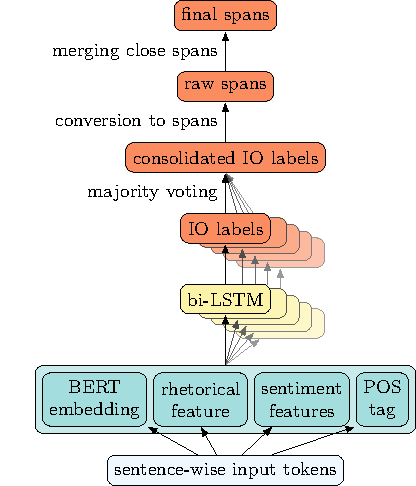
\includegraphics[width=1.25\textwidth,trim={5mm 0 0 0},clip]{task1-system.pdf}
\end{figure}
\end{column}
\begin{column}{0.155\paperwidth}
Embeddings
\begin{itemize}
    \item BERT base uncased \cite{devlin2019bert}
    \item (GloVe, small) \cite{pennington2014glove} 
\end{itemize}
Features
\begin{itemize}
    \item Match with rhetorically salient phrase patterns \cite{somasundaran2007detecting}
    \item Positive/negative sentiment \cite{baccianella2010sentiwordnet}
    \item POS tag \cite{spacy}
\end{itemize}
\end{column}
\end{columns}
\end{block}
\vspace{-0.6em}
\begin{alertblock}{Results}
Character-level F1: 43.9\% (rank 8/35); recall $>$ precision\\
(Corrected evaluation:* 43.6\%; 12/35)
% \begin{itemize}
%     \item GloVe (low precision, high recall) vs. BERT (higher precision, lower recall, higher F1)% \textrightarrow{} combined model would be interesting
%     \item Linguistic features: raise precision (at the cost of some recall)
%     \item Majority voting: raises precision, more stable performance
%     \item Span merging: raises precision and recall
% \end{itemize}
\begin{itemize}
    \item GloVe (recall$\uparrow$, precision$\downarrow$) vs. BERT (recall$\downarrow$, precision$\uparrow$, F1$\uparrow$)% \textrightarrow{} combined model would be interesting
    \item Features: precision$\nearrow$ (at the cost of some recall)
    \item Majority voting: precision$\nearrow$, more stable performance
    \item Span merging: recall$\nearrow$
\end{itemize}
\end{alertblock}
\end{column}
    
%----------------------------------------------------------------------------------------

\begin{column}{\sepwid}\end{column} % Empty spacer column
\begin{column}{\onecolwid}\vspace{\doublecoltopmargin}
\vspace{-0.6em}
\begin{exampleblock}{\vspace*{-1ex}}
\sethlcolor{paleyellow}
\overtext{\hl{it's inevitable that this bacterial infection}}{\normalsize Repetition} [...] will become resistant to antibiotics. [...]
But experts warn that [...]
\hl{antibiotics resistance is inevitable}
and
\sethlcolor{paleorange}
\undertext{\hl{making this disease much more terrifying.}}{\normalsize Appeal to fear/prejudice}
\end{exampleblock}
\vspace{1em}

\begin{block}{Identifying propaganda techniques}
\vspace{-0.2em}
\begin{figure}
    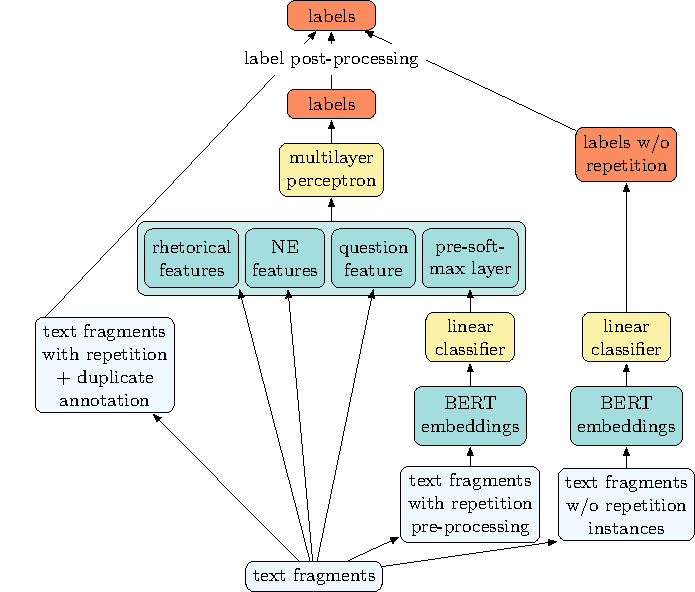
\includegraphics[width=1\textwidth,trim={6mm 0 0 0},clip]{task2-system.pdf}
\end{figure}
\vspace{0.2em}
\begin{itemize}
    \item Repetition pre-processing: Enhance fragments with 'repetition' label (train) or that appear elsewhere in the same article (dev/test) with duplicate
    \item Repetition post-processing: Classify \textbf{all} duplicates of a fragment within an article as `repetition'
    \item Additional model predicts extra label for instances with 2+~classes
\end{itemize}
\end{block}
\end{column}
\end{columns}
% Including footnotes in a beamer poster is complicated...
{\normalsize *The shared task's evaluation script contained a bug that was fixed after the competition ended.}
\end{column} 

\begin{column}{\sepwid}\end{column} % Empty spacer column
\begin{column}{\onecolwid}\vspace{\singlecoltopmargin}
\begin{block}{Identifying propaganda techniques cont'd}
\begin{itemize}
    \item Embeddings: BertForSequenceClassification \cite{Wolf2019HuggingFacesTS}\\%base uncased
    \item Classifier: MLP (SVM, linear classifier)
\end{itemize}
Features
\begin{itemize}
    \item Phrase pattern in rhetorical lexicon \cite{somasundaran2007detecting}
    \item Nationality/religion, country/city \cite{spacy}
    \item Question mark
    \item (More named entities, emotion \cite{emotion}, sequence length, \#~of repetitions)
\end{itemize}
\begin{alertblock}{Results}
Micro F1: 57.4\% (rank 8/31)\\
(Corrected evaluation:* 58.9\%; 6/31)
\begin{itemize}
    \item Repetition pre- and postprocessing: 
    % significantly raise~F1
    F1$\uparrow$
    \item Classifier choice: minor effect
    \item (Some) feature combinations: 
    % more stable performance, 
    % slightly raise~F1
    stability$\nearrow$,~F1$\nearrow$
\end{itemize}
\end{alertblock}
\end{block}

% \begin{block}{Further results \& discussion}
% \begin{itemize}
%     \item Both tasks: better performance on large classes
%     \item Decrease in repetition prediction (dev $>$ test; all teams)
% \end{itemize}
% \end{block}
\vspace{-2em}
\begin{block}{References}
\small{\bibliographystyle{unsrtetal}
\bibliography{lib}\vspace{0.75in}}
\end{block}


%----------------------------------------------------------------------------------------

\end{column} % End of the third column
\begin{column}{\sepwid}\end{column} % Empty spacer column
\end{columns} % End of all the columns in the poster
\end{frame} % End of the enclosing frame
\end{document}
